\documentclass[border=3pt,tikz]{standalone}
\usepackage{amsmath}
\usetikzlibrary{calc}
\usetikzlibrary{arrows.meta} % for arrow size
\begin{document}


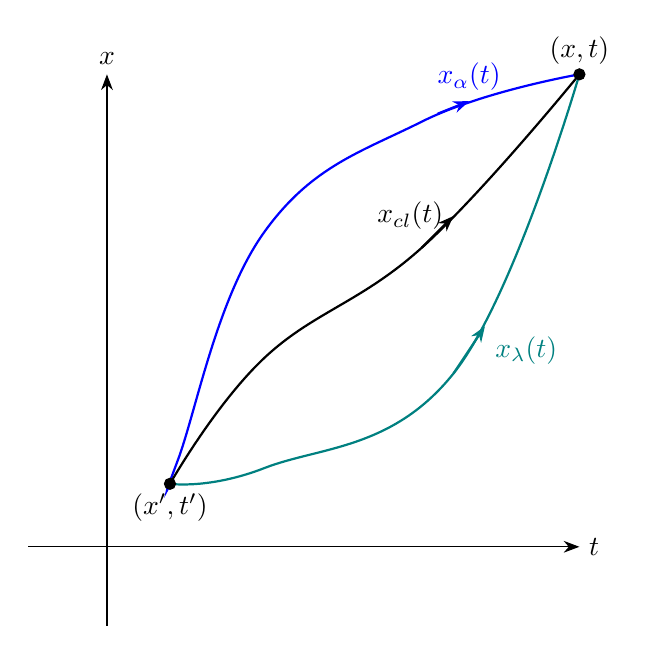
\begin{tikzpicture}[scale=2]
\usetikzlibrary {arrows.meta}
\usetikzlibrary {calc}


\draw[, -{Stealth[length=2mm]}] (-0.5, 0) -- (3, 0) node [right] {$t$} ;
\draw[, -{Stealth[length=2mm]}] (0, -0.5) -- (0, 3) node [above] {$x$};

\draw [blue, thick] plot [smooth, tension=0.7] coordinates { (0.4,0.4) (0.45, 0.55) (1,2) (2,2.7) (3,3)};
\draw [black, thick] plot [smooth, tension=0.7] coordinates { (0.4,0.4)  (1,1.2) (2,1.9) (3,3)};
\draw [teal, thick] plot [smooth, tension=0.7] coordinates { (0.4,0.4)  (1,0.5) (2.2,1.1) (3,3)};

\filldraw[black] (0.4, 0.4) circle (1pt) node[below] {$(x',t')$} ;
\filldraw[black] (3, 3) circle (1pt) node[above] {$(x,t)$} ;

\draw[blue, thick, -{Stealth[length=2mm]}] (2.1,2.75) -- (2.3, 2.83) node [above] {$x_\alpha(t)$} ;
\draw[black, thick, -{Stealth[length=2mm]}] (2.0,1.9) -- (2.2, 2.10) node [above, left] {$x_{cl}(t)$} ;

\draw[teal, thick, -{Stealth[length=2mm]}] (2.2,1.1) -- (2.4, 1.4) node [below right] {$x_\lambda(t)$} ;
\end{tikzpicture}
\end{document}